\documentclass{../../../../style/mkimain}

\series{2}
\month{březen}
\year{2023}

\begin{document}
\section*{II.K Není všechno teplé, co se třpytí!}
V minulém díle jsme si představili základní principy kvantového světa.
Vědní obor zabývající se popisem tohoto světa elementárních částic se nejčastěji nazývá jako \textit{kvantová mechanika}.
Nyní se však vydáme na cestu napříč časem i prostorem a podíváme se na historický vývoj tohoto odvětví fyziky.
Vysvětlíme si, proč byl vznik kvantové teorie potřeba a na základě čeho dostala své jméno.
\\

Naše putování můžeme začít v polovině 19. století,
kdy světoznámý fyzik \textit{James Clerk Maxwell} formuloval své čtyři základní rovnice elektromagnetismu.
Tyto rovnice se dodnes používají k popisu všech možných jevů a modelů jako je elektromagnetická indukce,
pole permanentního magnetu nebo třeba šíření světla.
A právě o světle bude v tomto seriálu řeč.

Z řešení Maxwellových rovnic vyplývá, že světlo se chová jako nositel elektromagnetického pole s vlnovým charakterem.
Pomocí Maxwellových rovnic se dokázalo to, co bylo téměř 200 let pozorováno. Světlo se šíří ve vlnách.

Vlnový popis světla se zdál být dostatečný,
a proto se na jeho základu snažili fyzici na přelomu 19. a 20. století postavit kompletní teorii vyzařování těles.
Lidé si v té době kladli otázky typu: proč hvězdy svítí?
Jakým mechanismem mohou ztrácet energii? Jak může těleso předávat teplo i bez kontaktu? Načež se dopracovalo k tomu,
že každé těleso, ať se nachází ve vakuu či atmosféře, musí odevzdávat teplo okolí.
Tento proces zprostředkovává právě ono elektromagnetické záření.
Každé těleso tedy dle teorie z konce 19. století jakýmsi způsobem \uv{svítí}.
Ale vzhledem k tomu, že ku příkladu lidi vidíme zářit maximálně tak v televizních výstupech,
může se tato teorie zdát jako trochu přitažená za vlasy.
Bylo proto potřeba spočítat, jak tomu doopravdy je.

Způsob, jak dosáhnout zpracovatelných dat,
je sestavit závislost tzv. \textit{spektrální intenzity záření} (míra vyzařování) na vlnové délce (vzdálenost mezi dvěma vrcholy světelné vlny).
Dle klasické fyziky bylo spočítáno, že spektrální intenzita by enormně rostla se zmenšující se vlnovou délkou.
Rostla by pořád a do nekonečna, což by nám říkalo, že tělesa by na ultrafialovém spektru vydávala nekonečně mnoho energie,
a to je samozřejmě nesmysl.
Tento problém nese věhlasné jméno \textit{ultrafialová katastrofa}.

Jak se s tímto problémem vypořádat? S touto otázkou zápasily koncem 19. století největší vědecké kapacity.
Ovšem teprve roku 1900 byla tato hádanka vyřešena a samozřejmě tento průlom neměl na svědomí nikdo jiný než sám německý fyzik \textit{Max Planck}.
Formuloval prvně z části odhadnutý, \textit{semiempirický} (z poloviny experimentálně zjištěný) vztah mezi spektrální intenzitou a vlnovou délkou.
O pár měsíců později se mu podařilo tento zákon plně odvodit díky jistému matematickému obratu.
Ten spočívá v předpokladu,
že světlo jakožto forma energie nemůže být vyzařováno spojitě či kontinuálně, nýbrž po určitých částech, tzv. \textit{kvantech}.
Takové \uv{balíčky} světelné energie dostaly název \textit{fotony}.
U takového modelu světla se může zdát, že je v nesouladu s vlnovým charakterem, jenže pouze tímto trikem lze dosáhnout správných výsledků.
Ukazuje nám to, že oba pohledy na povahu světla jsou správné, chová se jako částice a zároveň jako vlna.
O tomto paradoxu kvantové mechaniky se budeme podrobněji bavit příště. Na závěr zmiňuji,
že vyzařovací zákon formulovaný Planckem se dnes nazývá \textit{Planckův vyzařovací zákon} a jeho hlavní poselství je,
že každé těleso o libovolné teplotě vyzařuje na všech možných vlnových délkách, ovšem na některých více a na některých méně.
Jak moc na jakých vlnových délkách je už otázka teploty. Takže v podstatě i my sami záříme podobně jako Slunce viditelným světlem,
jenže tak nepatrně, že tento děj nelze postřehnout.
\\

Jistě jste si všimli, že jsme během vysvětlování podstaty světla použili slovo \textit{kvantum}.
A právě výše zmíněné použití tohoto slova vedlo ke vzniknu názvu \textit{kvantová fyzika}.
Hledání nejmenší možné části jisté veličiny (nejen energie, ale i další) se stalo podstatnou technikou tohoto revolučního oboru,
a fyzici proto pro něj vytvořili speciální název: \textit{kvantování}.
Jak následně ukázal všem známý Albert Einstein, kvantování není pouze matematický konstrukt, ale reálný jev přírody.
\\
\\
\begin{center}
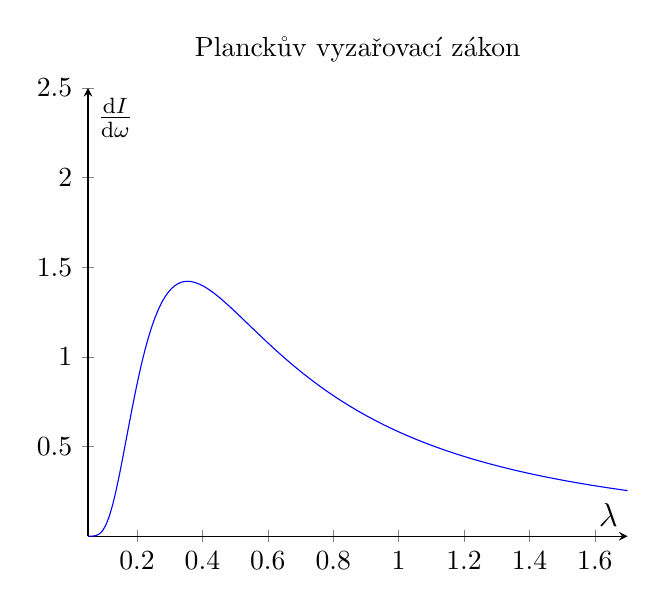
\begin{tikzpicture}
\begin{axis}[
    xmin=0.05, 
    xmax=1.7, 
    ymin=0, 
    ymax=2.5, 
    axis lines=middle, 
    xlabel=$\lambda$, 
    ylabel=$\frac{\mathrm{d}I}{\mathrm{d}\omega}$, 
    title={Planckův vyzařovací zákon}, 
    restrict y to domain=-1:2.5,
    label style={font=\large}]
\addplot[color=blue, samples=1000]{x^(-3)*(exp(x^(-1))-1)^(-1)};
\end{axis}
\end{tikzpicture}
\end{center}
\textbf{Úloha:}
\\
\\
Dle Planckova vyzařovacího zákona má závislost spektrální intenzity na vlnové délce jedno maximum.
V praxi to znamená, že tělesa vyzařují na všech vlnových délkách, ovšem na některých vyzařují méně a na některých více.
Existuje však jedna vlnová délka, na které dané těleso vyzařuje nejvíce, říkejme jí $\lambda_\mathrm{max}$.
A právě tuto vlnovou délku $\lambda_\mathrm{max}$ také nejlépe vidíme.
\begin{enumerate}
    \item Jaký je vztah mezi $\lambda_\mathrm{max}$ a teplotou příslušného tělesa?
    \begin{enumerate}[a)]
        \item $\lambda_\mathrm{max}$ je přímo úměrná teplotě tělesa
        \item $\lambda_\mathrm{max}$ je nepřímo úměrná teplotě tělesa
    \end{enumerate}
    \item Svou předchozí odpověd se pokuste zdůvodnit úvahou nebo prokázat na nějakém jevu v přírodě.
    \\\\
    \emph{Nápověda}: Zamyslete se například nad tím, co dává hvězdám jejich barvu.
    \item Jak se nazývá zákon, který dává do vztahu $\lambda_\mathrm{max}$ a teplotu vyzařujícího tělesa?
    \begin{enumerate}[a)]
        \item Stefan–Boltzmannův zákon
        \item De Broglieho vlna
        \item Einsteinova rovnice fotoefektu
        \item Wienův posunovací zákon
    \end{enumerate} 
\end{enumerate}
\end{document}
